% =============================================================================
%  Diplomado en Data Science Aplicada con Python para la Toma de Decisiones
%  Clase 19: Gradio + Aprendizaje No Supervisado (K-Means)
%  Arca Continental Ecuador | UDLA
%
%  Compilar: pdflatex -shell-escape presentacion.tex (x2 para refs)
% =============================================================================
\documentclass[aspectratio=169, 11pt]{beamer}

\usepackage[T1]{fontenc}
\usepackage[utf8]{inputenc}
\usepackage[spanish,es-noshorthands]{babel}
\usepackage{FiraSans}
\usepackage{FiraMono}
\renewcommand{\familydefault}{\sfdefault}
\usepackage{graphicx}
\usepackage{tikz}
\usetikzlibrary{arrows.meta, positioning, shapes.geometric, shapes.misc,
  calc, fit, decorations.pathreplacing, backgrounds}
\usepackage{fontawesome5}
\usepackage{minted}
\usepackage{tcolorbox}
\tcbuselibrary{minted, skins, breakable}
\usepackage{booktabs}
\usepackage{colortbl}
\usepackage{multicol}
\usepackage{hyperref}
\usepackage{calc}
\usepackage{amsmath}

\definecolor{arcaRed}{HTML}{C82B40}
\definecolor{arcaDark}{HTML}{6B1525}
\definecolor{udlaCrimson}{HTML}{A31545}
\definecolor{arcaGray}{HTML}{F5F5F5}
\definecolor{arcaLightGray}{HTML}{EBEBEB}
\definecolor{textDark}{HTML}{2D2D2D}
\definecolor{textMuted}{HTML}{6B7280}
\definecolor{codeGreen}{HTML}{16A34A}
\definecolor{codeBlue}{HTML}{2563EB}
\definecolor{codeOrange}{HTML}{EA580C}
\definecolor{codePurple}{HTML}{7C3AED}

\usetheme{default}
\usecolortheme{default}
\setbeamertemplate{navigation symbols}{}
\setbeamertemplate{footline}{}
\setbeamertemplate{headline}{}
\setbeamercolor{normal text}{fg=textDark}
\setbeamercolor{frametitle}{fg=arcaRed, bg=white}
\setbeamercolor{title}{fg=white}
\setbeamercolor{subtitle}{fg=white!85}
\setbeamercolor{author}{fg=white!80}
\setbeamercolor{date}{fg=white!70}
\setbeamercolor{item}{fg=arcaRed}
\setbeamercolor{subitem}{fg=arcaDark}
\setbeamercolor{block title}{fg=white, bg=arcaRed}
\setbeamercolor{block body}{fg=textDark, bg=arcaGray}
\setbeamercolor{block title alerted}{fg=white, bg=codeOrange}
\setbeamercolor{block body alerted}{fg=textDark, bg=arcaGray}
\setbeamercolor{block title example}{fg=white, bg=codeGreen}
\setbeamercolor{block body example}{fg=textDark, bg=arcaGray}
\setbeamercolor{section in toc}{fg=arcaDark}
\setbeamerfont{frametitle}{size=\Large, series=\bfseries}
\setbeamerfont{title}{size=\huge, series=\bfseries}
\setbeamerfont{subtitle}{size=\large}
\setbeamerfont{author}{size=\normalsize}
\setbeamerfont{date}{size=\small}
\setbeamerfont{block title}{size=\normalsize, series=\bfseries}
\setbeamerfont{footnote}{size=\tiny}
\setbeamertemplate{itemize item}{\scriptsize\raise1.5pt\hbox{\color{arcaRed}$\blacktriangleright$}}
\setbeamertemplate{itemize subitem}{\scriptsize\raise1pt\hbox{\color{arcaDark}$\bullet$}}
\setbeamertemplate{enumerate items}[default]
\setbeamercolor{enumerate item}{fg=arcaRed}

\setbeamertemplate{headline}{%
  \begin{tikzpicture}[remember picture, overlay]
    \fill[arcaDark] (current page.north west) rectangle
      ([yshift=-0.7cm]current page.north east);
    \node[anchor=west, inner sep=0pt] at
      ([xshift=0.6cm, yshift=-0.35cm]current page.north west)
      {
\includegraphics[height=0.45cm]{../logo_udla_white.png}};
    \node[anchor=east, inner sep=0pt] at
      ([xshift=-0.6cm, yshift=-0.35cm]current page.north east)
      {
\includegraphics[height=0.45cm]{../ArcaContinental_white.png}};
  \end{tikzpicture}%
  \vspace{0.7cm}%
}

\setbeamertemplate{footline}{%
  \begin{tikzpicture}[remember picture, overlay]
    \node[anchor=south east, font=\scriptsize\bfseries\color{arcaRed}] at
      ([xshift=-0.5cm, yshift=0.15cm]current page.south east)
      {\insertframenumber};
  \end{tikzpicture}%
  \vspace{0.3cm}%
}

\setbeamertemplate{frametitle}{%
  \vspace{0.25cm}%
  \usebeamerfont{frametitle}\usebeamercolor[fg]{frametitle}\insertframetitle%
  \par\vspace{2pt}%
  \begin{tikzpicture}
    \fill[arcaRed] (0,0) rectangle (3cm, 1.5pt);
    \fill[arcaLightGray] (3cm,0) rectangle (\textwidth, 0.5pt);
  \end{tikzpicture}%
  \vspace{0.1cm}%
}

\newtcblisting{pyblock}[1][]{%
  listing engine=minted, minted language=python, minted style=friendly,
  minted options={fontsize=\small, linenos=false, breaklines=true, python3=true},
  colback=arcaGray, colframe=arcaRed, left=4pt, right=4pt, top=4pt, bottom=4pt,
  boxrule=0pt, leftrule=3pt, arc=2pt, listing only, #1}

\newtcblisting{outputblock}[1][]{%
  listing engine=minted, minted language=text, minted style=bw,
  minted options={fontsize=\small, breaklines=true},
  colback=white, colframe=arcaLightGray, left=4pt, right=4pt, top=4pt, bottom=4pt,
  boxrule=0.5pt, arc=2pt, listing only,
  title={\small\faTerminal\hspace{6pt}Output}, coltitle=textMuted,
  fonttitle=\small\ttfamily, colbacktitle=white, #1}

\newcommand{\sectionframe}[2]{%
  \begingroup
  \setbeamertemplate{headline}{}%
  \setbeamertemplate{footline}{}%
  \begin{frame}[plain, noframenumbering]
    \begin{tikzpicture}[remember picture, overlay]
      \fill[arcaRed] (current page.south west) rectangle (current page.north east);
      \node[anchor=center, text=white, font=\Huge\bfseries, text width=12cm,
            align=center] at ([yshift=0.5cm]current page.center) {#1};
      \node[anchor=center, text=white!80, font=\large, text width=10cm,
            align=center] at ([yshift=-0.8cm]current page.center) {#2};
    \end{tikzpicture}
  \end{frame}
  \endgroup
}

\title{Diplomado en Data Science Aplicada\\con Python para la Toma de Decisiones}
\subtitle{Clase 19: Gradio + Aprendizaje No Supervisado (K-Means)}
\author{Carlos Enrique Mosquera Trujillo}
\date{27 de Abril, 2026}

\begin{document}

% ── PORTADA ──────────────────────────────────────────────────────────────────
{
\setbeamertemplate{headline}{}
\setbeamertemplate{footline}{}
\begin{frame}[plain, noframenumbering]
  \begin{tikzpicture}[remember picture, overlay]
    \fill[arcaDark] (current page.south west) rectangle (current page.north east);
    \fill[arcaRed] ([yshift=-3.5cm]current page.north west) rectangle
      ([yshift=-4.2cm]current page.north east);
    \node[anchor=west, inner sep=0pt] at
      ([xshift=1cm, yshift=-1.5cm]current page.north west)
      {
\includegraphics[height=1cm]{../logo_udla_white.png}};
    \node[anchor=east, inner sep=0pt] at
      ([xshift=-1cm, yshift=-1.5cm]current page.north east)
      {
\includegraphics[height=1cm]{../ArcaContinental_white.png}};
  \end{tikzpicture}
  \vspace{2.5cm}
  \begin{center}
    {\usebeamerfont{title}\usebeamercolor[fg]{title}\inserttitle\par}
    \vspace{0.4cm}
    {\usebeamerfont{subtitle}\usebeamercolor[fg]{subtitle}\insertsubtitle\par}
    \vspace{0.6cm}
    {\usebeamerfont{author}\usebeamercolor[fg]{author}\insertauthor\par}
    \vspace{0.15cm}
    {\usebeamerfont{date}\usebeamercolor[fg]{date}\insertdate\par}
  \end{center}
\end{frame}
}

% ── MÓDULO 4 ─────────────────────────────────────────────────────────────────
{
\setbeamertemplate{headline}{}
\setbeamertemplate{footline}{}
\begin{frame}[plain, noframenumbering]
  \begin{tikzpicture}[remember picture, overlay]
    \fill[arcaDark] (current page.south west) rectangle (current page.north east);
    \node[anchor=center, text=white, font=\Large\bfseries, text width=12cm,
          align=center] at ([yshift=1cm]current page.center)
      {M\'odulo 4 --- clase 6};
    \node[anchor=center, text=white!90, font=\huge\bfseries, text width=12cm,
          align=center] at ([yshift=-0.3cm]current page.center)
      {Machine Learning};
  \end{tikzpicture}
\end{frame}
}

% ── ROADMAP ─────────────────────────────────────────────────────────────────
\begin{frame}[shrink=22]{Hoja de Ruta de Hoy}
  \vspace{-4pt}
  \begin{center}
  \begin{tikzpicture}[
    node distance=0.35cm,
    roadstep/.style={rectangle, rounded corners=4pt, draw=arcaRed, fill=arcaRed!8,
                 minimum width=11cm, minimum height=0.65cm,
                 font=\footnotesize\bfseries\color{arcaDark}, align=left,
                 text width=10cm, inner sep=6pt},
    num/.style={circle, fill=arcaRed, text=white, font=\scriptsize\bfseries,
                minimum size=0.5cm, inner sep=0pt},
  ]
    \node[roadstep] (s0) {\hspace{0.8cm}Despliegue de modelos: por qu\'e importa y qu\'e es una API};
    \node[roadstep, below=of s0] (s1) {\hspace{0.8cm}Gradio paso a paso: componentes, inputs, outputs, demo completa};
    \node[roadstep, below=of s1] (s2) {\hspace{0.8cm}Supervisado vs No Supervisado: un paradigma nuevo};
    \node[roadstep, below=of s2] (s3) {\hspace{0.8cm}K-Means: la intuici\'on, el algoritmo paso a paso};
    \node[roadstep, below=of s3] (s4) {\hspace{0.8cm}Elegir K: el m\'etodo del codo};
    \node[roadstep, below=of s4] (s5) {\hspace{0.8cm}Aplicaci\'on: segmentar clientes de un centro comercial};
    \node[roadstep, below=of s5] (s6) {\hspace{0.8cm}Interpretar los clusters: perfilar y nombrar cada segmento};

    \node[num] at ([xshift=0.45cm]s0.west) {1};
    \node[num] at ([xshift=0.45cm]s1.west) {2};
    \node[num] at ([xshift=0.45cm]s2.west) {3};
    \node[num] at ([xshift=0.45cm]s3.west) {4};
    \node[num] at ([xshift=0.45cm]s4.west) {5};
    \node[num] at ([xshift=0.45cm]s5.west) {6};
    \node[num] at ([xshift=0.45cm]s6.west) {7};
  \end{tikzpicture}
  \end{center}
\end{frame}

% =============================================================================
%  BLOQUE A: DESPLIEGUE DE MODELOS
% =============================================================================
\sectionframe{Despliegue de Modelos}{Del notebook al mundo real}

\begin{frame}{El Modelo en el Notebook No Sirve de Nada}
  \vspace{-4pt}
  {\footnotesize\color{arcaDark}\bfseries
    Como cient\'ificos de datos, nuestra responsabilidad \textbf{no termina}
    cuando el AUC es bueno. El modelo tiene que \textbf{llegar al usuario}.}

  \vspace{6pt}
  {\footnotesize
  \begin{itemize}\setlength{\itemsep}{5pt}
    \item[{\color{arcaRed}\scriptsize\faTimesCircle}]
      Un notebook en tu laptop no le sirve al m\'edico que eval\'ua
      pacientes a las 3am.
    \item[{\color{arcaRed}\scriptsize\faTimesCircle}]
      Un archivo \texttt{.pkl} no le dice nada al gerente.
    \item[{\color{codeGreen}\scriptsize\faCheckCircle}]
      Lo que necesitan es una \textbf{interfaz}: algo donde ingresen datos
      y vean el resultado.
  \end{itemize}
  }

  \vspace{6pt}
  \begin{tcolorbox}[colback=arcaGray, colframe=arcaRed, boxrule=0.5pt, arc=2pt,
    left=6pt, right=6pt, top=4pt, bottom=4pt]
    {\scriptsize\color{arcaDark}
    \faKey\hspace{4pt}\textbf{Desplegar} (deploy) = poner el modelo en un
    lugar donde otras personas puedan usarlo sin saber Python.
    El despliegue es parte del trabajo del data scientist.}
  \end{tcolorbox}
\end{frame}

\begin{frame}{?`Qu\'e Es una API?}
  \vspace{-4pt}
  {\footnotesize\color{arcaDark}\bfseries
    API = Application Programming Interface. Es un \textbf{contrato}
    entre dos sistemas: ``si me mandas estos datos, te devuelvo esto''.}

  \vspace{6pt}
  {\footnotesize
  \begin{itemize}\setlength{\itemsep}{5pt}
    \item[{\color{arcaRed}\scriptsize\faArrowRight}]
      Cuando usan Google Maps en una app, la app le \textbf{manda}
      coordenadas a la API de Google, y la API le \textbf{devuelve} un mapa.
    \item[{\color{arcaRed}\scriptsize\faArrowRight}]
      Cuando una app de banco muestra su saldo, la app le
      \textbf{manda} su ID a la API del banco, y la API
      \textbf{devuelve} el n\'umero.
    \item[{\color{codeGreen}\scriptsize\faArrowRight}]
      Nuestros modelos pueden funcionar igual: alguien \textbf{manda}
      datos de un paciente, la API \textbf{devuelve} la predicci\'on.
  \end{itemize}
  }

  \vspace{6pt}
  {\scriptsize\color{textMuted}
    \faLightbulb\hspace{4pt} El patr\'on siempre es el mismo:
    \textbf{input $\to$ funci\'on $\to$ output}. Gradio, Streamlit,
    FastAPI --- todos hacen exactamente eso.}
\end{frame}

\begin{frame}{Opciones para Desplegar}
  \vspace{-4pt}
  {\scriptsize
  \begin{tabular}{@{}lp{4cm}p{2.5cm}p{3.5cm}@{}}
    \toprule
    \textbf{Herramienta} & \textbf{?`Qu\'e produce?} & \textbf{Complejidad} & \textbf{Cu\'ando usarla} \\
    \midrule
    \textbf{\color{codePurple}Gradio} & Interfaz web desde Jupyter. & 5--10 l\'ineas. & Demos, prototipos. \\
    \textbf{Streamlit} & App web/dashboard. & 30--80 l\'ineas. & Dashboards internos. \\
    \textbf{Flask / FastAPI} & API REST (JSON). & 100+ l\'ineas. & Producci\'on real. \\
    \textbf{Docker + Cloud} & Servicio escalable. & Infraestructura. & Miles de usuarios. \\
    \bottomrule
  \end{tabular}
  }

  \vspace{8pt}
  \begin{tcolorbox}[colback=codePurple!8, colframe=codePurple, boxrule=0.5pt, arc=2pt,
    left=6pt, right=6pt, top=4pt, bottom=4pt]
    {\scriptsize\color{arcaDark}
    \faLightbulb\hspace{4pt}\textbf{Hoy usamos Gradio}: la barrera de entrada
    m\'as baja. Funciona dentro de Jupyter, no necesita servidor.
    Si despu\'es necesitan algo m\'as robusto, la migraci\'on es natural
    porque el patr\'on (input $\to$ funci\'on $\to$ output) es el mismo.}
  \end{tcolorbox}
\end{frame}

% =============================================================================
%  BLOQUE B: GRADIO PASO A PASO
% =============================================================================
\sectionframe{Gradio}{Paso a paso --- de lo m\'as simple a lo complejo}

\begin{frame}[fragile,shrink=10]{Ejemplo 1: Una Funci\'on que Saluda}
  \vspace{-4pt}
  {\footnotesize\color{arcaDark}\bfseries
    Empecemos con lo m\'as b\'asico posible: una funci\'on que
    recibe un nombre y devuelve un saludo.}

  \vspace{4pt}
  \begin{pyblock}
import gradio as gr

def saludar(nombre):
    return f"Hola, {nombre}! Bienvenido al diplomado."

demo = gr.Interface(fn=saludar,
                    inputs="text",
                    outputs="text")
demo.launch()
  \end{pyblock}

  \vspace{4pt}
  {\scriptsize\color{arcaDark}
    \faKey\hspace{4pt} Tres piezas: \texttt{fn} (la funci\'on Python),
    \texttt{inputs} (qu\'e recibe), \texttt{outputs} (qu\'e devuelve).
    Gradio genera la interfaz web autom\'aticamente.}
\end{frame}

\begin{frame}[fragile,shrink=10]{Ejemplo 2: Multiplicar Dos N\'umeros}
  \vspace{-4pt}
  {\footnotesize\color{arcaDark}\bfseries
    Ahora con dos entradas num\'ericas:}

  \vspace{4pt}
  \begin{pyblock}
def multiplicar(a, b):
    return a * b

demo = gr.Interface(
    fn=multiplicar,
    inputs=[gr.Number(label="Numero A"),
            gr.Number(label="Numero B")],
    outputs=gr.Number(label="Resultado"))
demo.launch()
  \end{pyblock}

  \vspace{4pt}
  {\scriptsize\color{arcaDark}
    \faArrowRight\hspace{4pt} Cuando hay \textbf{m\'ultiples inputs}, se pasan
    como una \textbf{lista}. Cada elemento de la lista es un par\'ametro
    de la funci\'on, en orden.}
\end{frame}

\begin{frame}[fragile,shrink=10]{Ejemplo 3: Slider + Dropdown}
  \vspace{-4pt}
  {\footnotesize\color{arcaDark}\bfseries
    Combinemos tipos de entrada distintos:}

  \vspace{4pt}
  \begin{pyblock}
def calcular_propina(monto, porcentaje, dividir_entre):
    propina = monto * (porcentaje / 100)
    total = monto + propina
    por_persona = total / dividir_entre
    return f"Propina: ${propina:.2f} | Total: ${total:.2f} | Por persona: ${por_persona:.2f}"

demo = gr.Interface(
    fn=calcular_propina,
    inputs=[
        gr.Slider(10, 500, value=100, label="Monto de la cuenta ($)"),
        gr.Slider(5, 30, value=15, step=1, label="Propina (%)"),
        gr.Dropdown([1,2,3,4,5,6], value=2, label="Dividir entre"),
    ],
    outputs="text",
    title="Calculadora de Propina")
demo.launch()
  \end{pyblock}
\end{frame}

\begin{frame}[shrink=5]{Componentes Disponibles}
  \vspace{-4pt}
  {\footnotesize\color{arcaDark}\bfseries
    Gradio tiene componentes para cada tipo de dato:}

  \vspace{6pt}
  {\scriptsize
  \begin{tabular}{@{}lll@{}}
    \toprule
    \textbf{Tipo de dato} & \textbf{Input} & \textbf{Output} \\
    \midrule
    N\'umero & \texttt{gr.Number()}, \texttt{gr.Slider()} & \texttt{gr.Number()} \\
    Texto & \texttt{gr.Textbox()} & \texttt{gr.Textbox()} \\
    Opci\'on & \texttt{gr.Dropdown()}, \texttt{gr.Radio()} & \texttt{gr.Label()} \\
    S\'i/No & \texttt{gr.Checkbox()} & --- \\
    Imagen & \texttt{gr.Image()} & \texttt{gr.Image()} \\
    Gr\'afico & --- & \texttt{gr.Plot()} \\
    Varios & lista de componentes & lista de componentes \\
    \bottomrule
  \end{tabular}
  }

  \vspace{6pt}
  {\scriptsize\color{textMuted}
    \faLightbulb\hspace{4pt} Para m\'ultiples outputs, la funci\'on retorna
    una tupla: \texttt{return texto, figura} y Gradio muestra ambos.}
\end{frame}

\begin{frame}[fragile,shrink=22]{Ejemplo 4: Predictor de Diabetes (el modelo real)}
  \vspace{-6pt}
  {\footnotesize\color{arcaDark}\bfseries
    Ahora s\'i --- conectemos Gradio con el modelo de la clase anterior:}

  \vspace{4pt}
  \begin{pyblock}
def predecir_diabetes(embarazos, glucosa, presion, pliegue,
                      insulina, bmi, pedigri, edad):
    paciente = pd.DataFrame([{
        "preg": embarazos, "plas": glucosa, "pres": presion,
        "skin": pliegue, "insu": insulina, "mass": bmi,
        "pedi": pedigri, "age": edad}])
    proba = rf.predict_proba(paciente)[0, 1]
    nivel = "ALTO" if proba >= 0.5 else "MEDIO" if proba >= 0.2 else "BAJO"
    return f"Riesgo de Diabetes: {proba:.1%} ({nivel})"

demo = gr.Interface(fn=predecir_diabetes,
    inputs=[gr.Slider(0,17,1,step=1,label="Embarazos"),
            gr.Slider(0,200,100,label="Glucosa"),
            gr.Slider(0,122,70,label="Presion"),
            gr.Slider(0,99,20,label="Pliegue cutaneo"),
            gr.Slider(0,846,80,label="Insulina"),
            gr.Slider(10,67,25,step=0.5,label="BMI"),
            gr.Slider(0,2.5,0.5,step=0.01,label="Pedigri"),
            gr.Slider(21,81,30,step=1,label="Edad")],
    outputs="text", title="Predictor de Diabetes")
demo.launch()
  \end{pyblock}
\end{frame}

\begin{frame}[fragile,shrink=10]{Compartir con \texttt{share=True}}
  \vspace{-4pt}
  {\footnotesize\color{arcaDark}\bfseries
    Una l\'inea m\'as y cualquier persona puede usar tu modelo:}

  \vspace{4pt}
  \begin{pyblock}
demo.launch(share=True)
# -> Running on public URL: https://xxxxx.gradio.live
  \end{pyblock}

  \vspace{6pt}
  {\footnotesize
  \begin{itemize}\setlength{\itemsep}{4pt}
    \item[{\color{codeGreen}\scriptsize\faCheckCircle}]
      Genera un \textbf{link p\'ublico temporal} (72 horas).
    \item[{\color{codeGreen}\scriptsize\faCheckCircle}]
      El m\'edico abre el link en su celular y prueba pacientes.
    \item[{\color{codeGreen}\scriptsize\faCheckCircle}]
      No necesita Python, no necesita instalar nada.
    \item[{\color{arcaRed}\scriptsize\faTimesCircle}]
      El link expira en 72h. Para producci\'on real: Hugging Face
      Spaces, Streamlit Cloud, o FastAPI + Docker.
  \end{itemize}
  }
\end{frame}

\begin{frame}[shrink=5]{Ejercicio 1: De lo Simple a lo Complejo}
  \vspace{-4pt}
  {\footnotesize\color{arcaDark}\bfseries
    \faClock\hspace{4pt} 15 minutos --- en el notebook:}

  \vspace{6pt}
  {\footnotesize
  \begin{enumerate}\setlength{\itemsep}{4pt}
    \item \texttt{!pip install gradio}
    \item Hagan el ejemplo del saludo. Lancen y prueben.
    \item Hagan el ejemplo de la multiplicaci\'on. Lancen y prueben.
    \item Hagan el predictor de diabetes con el RF entrenado.
    \item Prueben: paciente de 45 a\~nos, glucosa 180, BMI 35.
    \item Prueben: paciente de 25 a\~nos, glucosa 85, BMI 22.
    \item \textbf{Bonus:} \texttt{share=True} y compartan el link.
  \end{enumerate}
  }
\end{frame}

% =============================================================================
%  BLOQUE C: SUPERVISADO VS NO SUPERVISADO
% =============================================================================
\sectionframe{Aprendizaje No Supervisado}{Un paradigma completamente nuevo}

\begin{frame}{Hasta Ahora: Siempre Ten\'iamos la Respuesta}
  \vspace{-4pt}
  {\footnotesize\color{arcaDark}\bfseries
    En todas las clases anteriores (13--18) siempre ten\'iamos una
    columna \textbf{target} ($y$): diabetes s\'i/no, precio del seguro,
    riesgo de ACV.}

  \vspace{6pt}
  {\footnotesize
  \begin{itemize}\setlength{\itemsep}{5pt}
    \item[{\color{codeBlue}\scriptsize\faArrowRight}]
      El modelo aprende la relaci\'on $X \to y$ con ejemplos etiquetados.
    \item[{\color{codeBlue}\scriptsize\faArrowRight}]
      Evaluamos con m\'etricas claras: AUC, recall, precision.
    \item[{\color{codeBlue}\scriptsize\faArrowRight}]
      Sabemos si el modelo acert\'o o no.
  \end{itemize}
  }

  \vspace{6pt}
  {\footnotesize\color{arcaDark}\bfseries
    Pero en la vida real, muchas veces \textbf{no tenemos target}:}

  \vspace{4pt}
  {\footnotesize
  \begin{itemize}\setlength{\itemsep}{3pt}
    \item[{\color{arcaRed}\scriptsize\faArrowRight}]
      ``Tengo 10\,000 clientes. Quiero \textbf{agruparlos} en segmentos
      para hacer campa\~nas distintas. Pero nadie me dijo cu\'ales son
      los grupos.''
    \item[{\color{arcaRed}\scriptsize\faArrowRight}]
      ``Tengo transacciones. Quiero detectar las \textbf{an\'omalas}.
      Pero no tengo ejemplos de fraude etiquetados.''
  \end{itemize}
  }
\end{frame}

\begin{frame}[shrink=15]{Supervisado vs No Supervisado --- La Diferencia}
  \vspace{-4pt}
  \begin{center}
    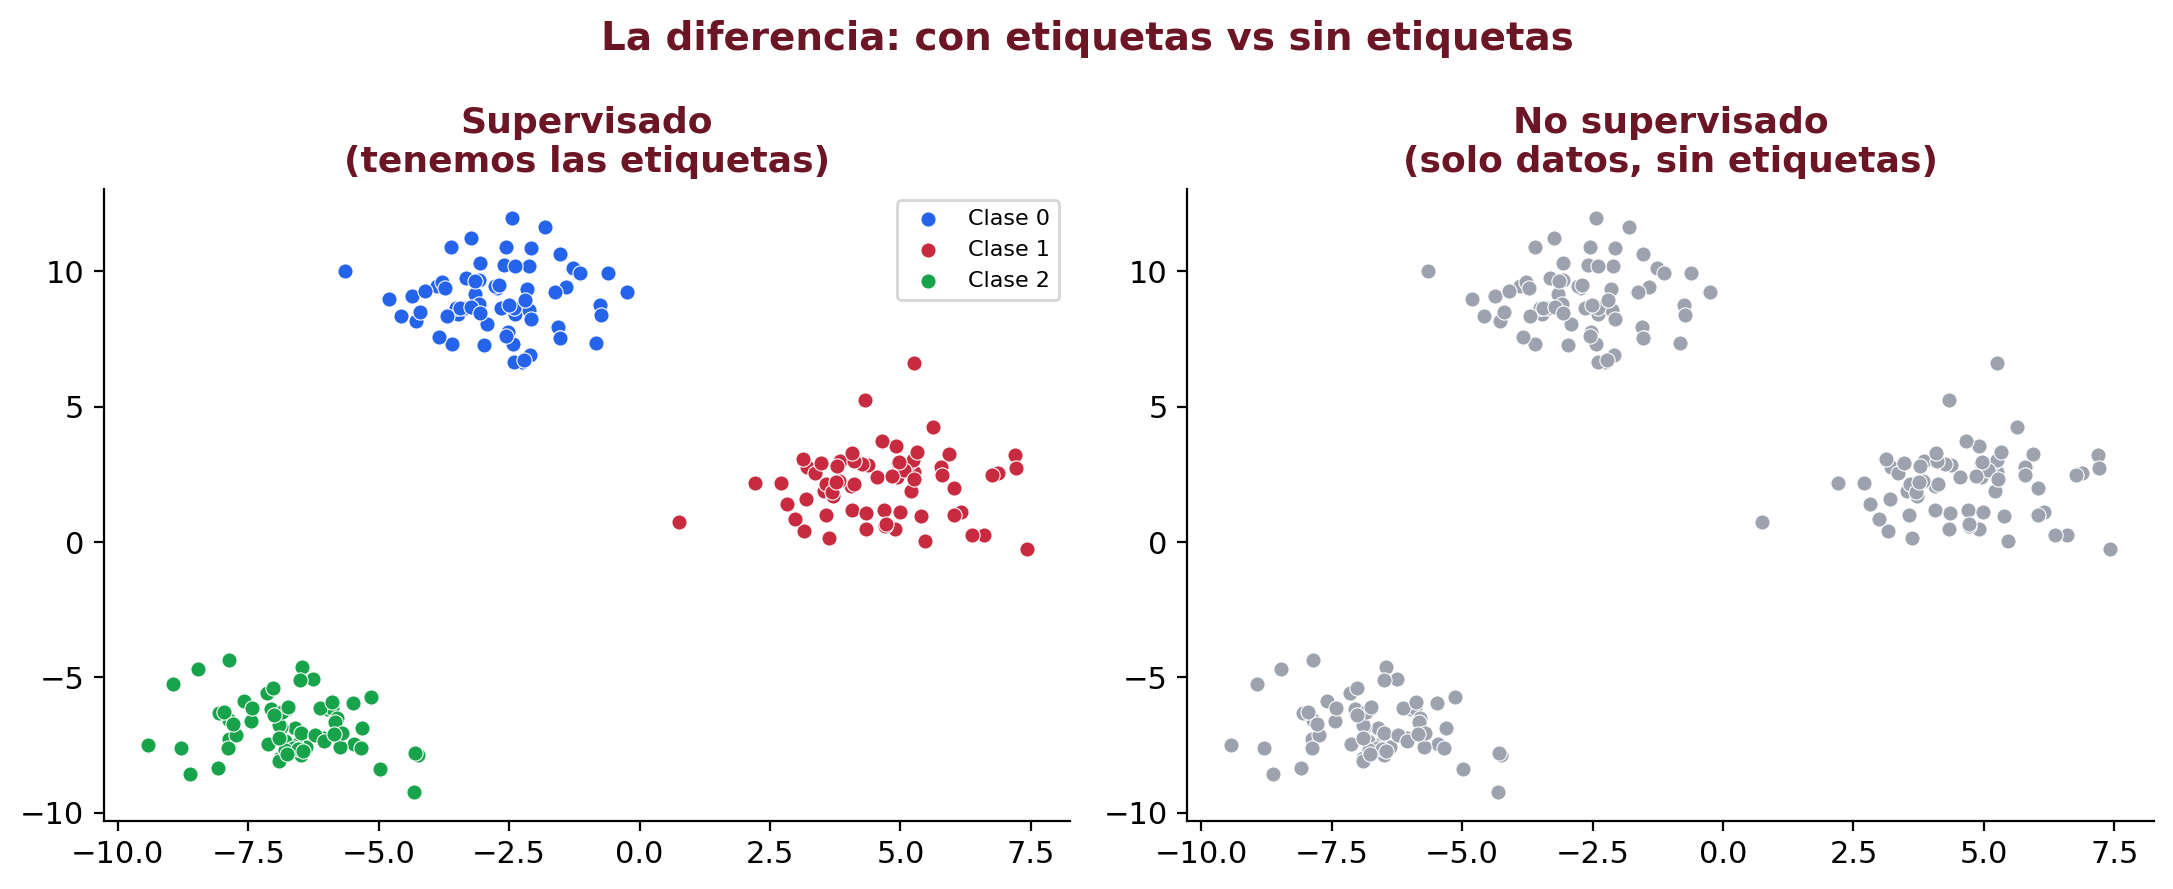
\includegraphics[width=0.88\textwidth]{fig_sup_vs_nosup.png}
  \end{center}

  \vspace{-2pt}
  {\scriptsize\color{textMuted}
    \faLightbulb\hspace{4pt} \textbf{Izquierda:} supervisado --- cada punto
    tiene un color (etiqueta). El modelo aprende qu\'e color asignar.
    \textbf{Derecha:} no supervisado --- todos los puntos son grises.
    El modelo debe \textit{descubrir} los grupos por s\'i solo.}
\end{frame}

\begin{frame}{?`Cu\'ando Usar Cada Uno?}
  \vspace{-4pt}
  {\scriptsize
  \begin{tabular}{@{}p{3cm}p{5cm}p{4.5cm}@{}}
    \toprule
     & \textbf{\color{codeBlue}Supervisado} & \textbf{\color{codePurple}No supervisado} \\
    \midrule
    \textbf{Datos} & Features + target ($y$). & Solo features ($X$). \\
    \textbf{Objetivo} & Predecir $y$ para datos nuevos. & Descubrir estructura oculta. \\
    \textbf{Evaluaci\'on} & AUC, recall, precision (claras). & M\'as subjetiva (no hay ``respuesta correcta''). \\
    \textbf{Ejemplos} & Clasificaci\'on, regresi\'on. & Clustering, reducci\'on de dimensiones. \\
    \textbf{Aplicaci\'on Arca} & ?`Este cliente va a comprar? & ?`Qu\'e tipos de clientes tenemos? \\
    \bottomrule
  \end{tabular}
  }

  \vspace{6pt}
  \begin{tcolorbox}[colback=codePurple!8, colframe=codePurple, boxrule=0.5pt, arc=2pt,
    left=6pt, right=6pt, top=4pt, bottom=4pt]
    {\scriptsize\color{arcaDark}
    \faKey\hspace{4pt}\textbf{No supervisado no reemplaza a supervisado.}
    Son herramientas complementarias. Muchas veces se usan juntas:
    primero segmentar (no sup.), luego predecir dentro de cada segmento (sup.).}
  \end{tcolorbox}
\end{frame}

% =============================================================================
%  BLOQUE D-pre: QU\'E ES SEGMENTAR + CU\'ANDO ES \'UTIL
% =============================================================================
\sectionframe{Segmentaci\'on}{?`Qu\'e significa y cu\'ando sirve?}

\begin{frame}{?`Qu\'e Significa Segmentar?}
  \vspace{-4pt}
  {\footnotesize\color{arcaDark}\bfseries
    Segmentar = dividir un grupo grande en \textbf{subgrupos m\'as
    peque\~nos y homog\'eneos}. Cada subgrupo comparte caracter\'isticas
    que lo hacen distinto de los dem\'as.}

  \vspace{8pt}
  {\footnotesize
  \begin{itemize}\setlength{\itemsep}{5pt}
    \item[{\color{arcaRed}\scriptsize\faArrowRight}]
      \textbf{Sin segmentar:} ``tenemos 200 clientes''. Todos reciben
      la misma promoci\'on, el mismo email, la misma atenci\'on.
    \item[{\color{codeGreen}\scriptsize\faArrowRight}]
      \textbf{Con segmentaci\'on:} ``tenemos 5 \textit{tipos} de clientes.
      Los premium reciben experiencias VIP. Los ahorradores reciben
      cupones de descuento. Los gastadores reciben programa de puntos.''
    \item[{\color{codeGreen}\scriptsize\faArrowRight}]
      La segmentaci\'on permite \textbf{personalizar} la estrategia.
      Es la diferencia entre hablarle a una multitud y hablarle
      a una persona.
  \end{itemize}
  }

  \vspace{4pt}
  {\scriptsize\color{textMuted}
    \faLightbulb\hspace{4pt} Segmentar no es clasificar. En clasificaci\'on
    las categor\'ias ya existen (diabetes s\'i/no). En segmentaci\'on
    \textbf{los grupos los descubre el algoritmo} a partir de los datos.}
\end{frame}

\begin{frame}{?`Cu\'ando Es \'Util Segmentar?}
  \vspace{-4pt}
  {\footnotesize\color{arcaDark}\bfseries
    Situaciones reales donde la segmentaci\'on genera valor:}

  \vspace{6pt}
  {\scriptsize
  \begin{tabular}{@{}p{3.5cm}p{4.5cm}p{4cm}@{}}
    \toprule
    \textbf{\'Area} & \textbf{Problema} & \textbf{Valor de segmentar} \\
    \midrule
    \textbf{Marketing} & 10\,000 clientes, presupuesto limitado. & Campa\~nas dirigidas: cada segmento recibe el mensaje correcto. \\
    \textbf{Retail / Arca} & Puntos de venta con comportamiento distinto. & Optimizar inventario y log\'istica por tipo de tienda. \\
    \textbf{Salud} & Pacientes con la misma enfermedad pero perfiles distintos. & Tratamientos diferenciados por perfil de riesgo. \\
    \textbf{Finanzas} & Clientes de un banco con patrones de uso variados. & Productos financieros personalizados. \\
    \textbf{RRHH} & Empleados con niveles de satisfacci\'on distintos. & Estrategias de retenci\'on por segmento. \\
    \bottomrule
  \end{tabular}
  }

  \vspace{6pt}
  \begin{tcolorbox}[colback=arcaGray, colframe=arcaRed, boxrule=0.5pt, arc=2pt,
    left=6pt, right=6pt, top=4pt, bottom=4pt]
    {\scriptsize\color{arcaDark}
    \faKey\hspace{4pt}\textbf{Regla pr\'actica:} si est\'as tratando a todos
    por igual y sospechas que hay subgrupos con necesidades distintas,
    la segmentaci\'on puede ayudarte. El algoritmo m\'as com\'un para esto
    es \textbf{K-Means}.}
  \end{tcolorbox}
\end{frame}

% =============================================================================
%  BLOQUE D: K-MEANS
% =============================================================================
\sectionframe{K-Means}{El algoritmo de clustering m\'as usado}

\begin{frame}{K-Means: La Idea en una Frase}
  \vspace{-4pt}
  {\footnotesize\color{arcaDark}\bfseries
    K-Means agrupa $N$ observaciones en $K$ grupos, de forma que
    cada observaci\'on pertenece al grupo cuyo \textbf{centro}
    (centroide) est\'a m\'as cerca.}

  \vspace{8pt}
  {\footnotesize
  \begin{itemize}\setlength{\itemsep}{5pt}
    \item[{\color{arcaRed}\scriptsize\faArrowRight}]
      $K$ lo elegimos \textbf{nosotros} (despu\'es veremos c\'omo).
    \item[{\color{arcaRed}\scriptsize\faArrowRight}]
      Un \textbf{centroide} es simplemente el \textbf{promedio} de
      todos los puntos de su grupo. Si 3 clientes tienen ingresos
      50, 60, 70 $\to$ centroide de ingreso = 60.
    \item[{\color{arcaRed}\scriptsize\faArrowRight}]
      ``M\'as cercano'' = menor \textbf{distancia euclidiana}
      (la l\'inea recta entre dos puntos en el espacio de variables).
  \end{itemize}
  }

  \vspace{6pt}
  {\scriptsize\color{textMuted}
    \faLightbulb\hspace{4pt} El objetivo: que los puntos dentro de un
    cluster sean lo m\'as \textbf{parecidos} entre s\'i y lo m\'as
    \textbf{diferentes} de los otros clusters.}
\end{frame}

\begin{frame}[fragile,shrink=10]{K-Means: El Pseudoc\'odigo}
  \vspace{-4pt}
  {\footnotesize\color{arcaDark}\bfseries
    El algoritmo completo en 8 l\'ineas legibles:}

  \vspace{4pt}
  \begin{pyblock}
K = 5   # nosotros elegimos cuantos grupos

# 1. Poner K centroides en posiciones aleatorias
centroides = elegir_K_puntos_al_azar(datos, K)

repetir hasta que nada cambie:
    # 2. Para cada punto, ver cual centroide esta mas cerca
    for punto in datos:
        punto.grupo = centroide_mas_cercano(punto, centroides)

    # 3. Mover cada centroide al promedio de sus puntos
    for k in range(K):
        centroides[k] = promedio(puntos del grupo k)
  \end{pyblock}

  \vspace{4pt}
  {\scriptsize\color{arcaDark}
    \faKey\hspace{4pt} Solo dos operaciones que se repiten:
    \textbf{asignar} (paso 2) y \textbf{recalcular} (paso 3).
    El algoritmo para cuando las asignaciones ya no cambian
    entre una iteraci\'on y la siguiente.}
\end{frame}

\begin{frame}[shrink=22]{K-Means Paso a Paso --- Visual}
  \vspace{-4pt}
  \begin{center}
    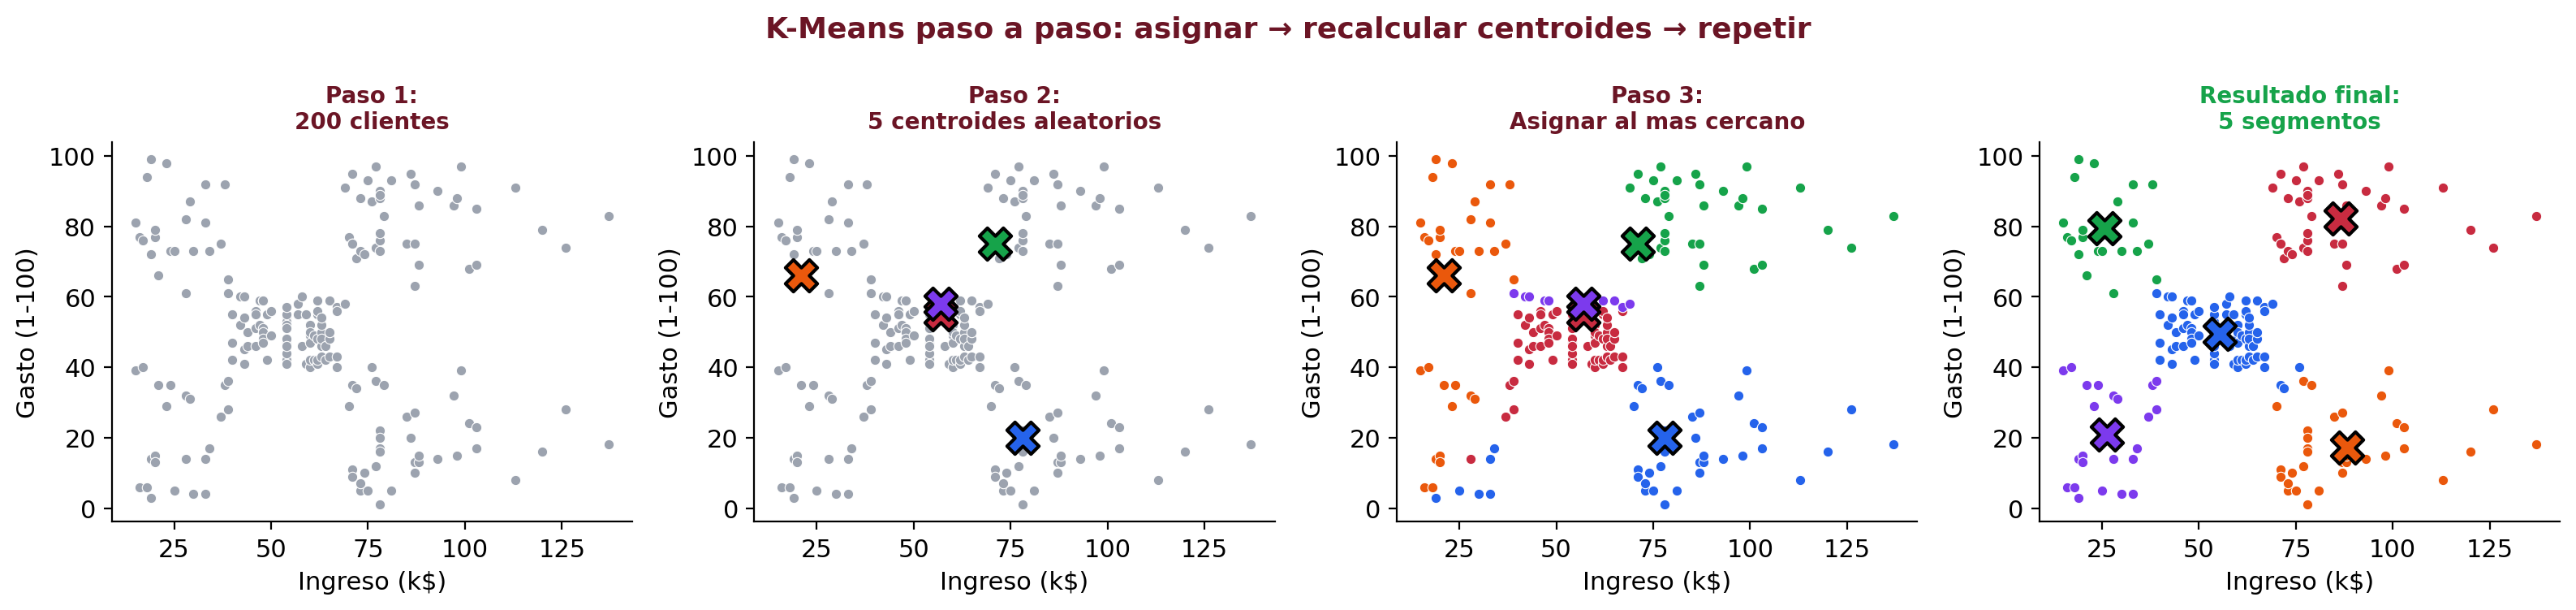
\includegraphics[width=0.95\textwidth]{fig_kmeans_pasos.png}
  \end{center}

  \vspace{-2pt}
  {\scriptsize\color{textMuted}
    \faLightbulb\hspace{4pt} \textbf{Paso 1:} datos sin color.
    \textbf{Paso 2:} centroides aleatorios (X grandes).
    \textbf{Paso 3:} cada punto toma el color del centroide m\'as cercano.
    \textbf{Paso 4:} despu\'es de iterar, los centroides se estabilizan.}
\end{frame}

\begin{frame}{?`Qu\'e Significa ``M\'as Cercano''?}
  \vspace{-4pt}
  {\footnotesize\color{arcaDark}\bfseries
    K-Means usa la \textbf{distancia euclidiana} --- la l\'inea recta
    entre dos puntos en el espacio de las variables.}

  \vspace{6pt}
  {\footnotesize
  \begin{itemize}\setlength{\itemsep}{5pt}
    \item[{\color{arcaRed}\scriptsize\faArrowRight}]
      Con 2 variables (ingreso, gasto): la distancia es la que
      medir\'ian con una regla en el scatter.
    \item[{\color{arcaRed}\scriptsize\faArrowRight}]
      Con 8 variables: la misma f\'ormula pero en 8 dimensiones.
      No la podemos visualizar, pero el c\'alculo es id\'entico.
    \item[{\color{arcaRed}\scriptsize\faArrowRight}]
      El \textbf{centroide} es simplemente el \textbf{promedio}
      de todas las observaciones del cluster. Si un cluster tiene
      3 clientes con ingresos 50, 60, 70 $\to$ centroide = 60.
  \end{itemize}
  }

  \vspace{4pt}
  {\scriptsize\color{textMuted}
    \faLightbulb\hspace{4pt} Por eso escalar importa: si ingreso va
    de 15 a 137 y gasto de 1 a 99, la distancia queda dominada por
    ingreso. \texttt{StandardScaler} pone ambas en la misma escala.}
\end{frame}

\begin{frame}{?`Cu\'ando Para el Algoritmo?}
  \vspace{-4pt}
  {\footnotesize\color{arcaDark}\bfseries
    K-Means itera hasta que se cumple una de estas condiciones:}

  \vspace{6pt}
  {\footnotesize
  \begin{itemize}\setlength{\itemsep}{5pt}
    \item[{\color{codeGreen}\scriptsize\faCheckCircle}]
      \textbf{Convergencia:} los centroides dejan de moverse
      (o se mueven menos de un umbral m\'inimo). Los clusters
      se estabilizaron.
    \item[{\color{arcaRed}\scriptsize\faCheckCircle}]
      \textbf{M\'aximo de iteraciones:} por defecto sklearn usa 300.
      Si no converge, para igual y devuelve el mejor resultado.
  \end{itemize}
  }

  \vspace{6pt}
  \begin{tcolorbox}[colback=arcaGray, colframe=arcaRed, boxrule=0.5pt, arc=2pt,
    left=6pt, right=6pt, top=4pt, bottom=4pt]
    {\scriptsize\color{arcaDark}
    \faExclamationTriangle\hspace{4pt}\textbf{Importante:} el resultado
    depende de los centroides iniciales (aleatorios). Por eso sklearn
    corre K-Means \textbf{10 veces} (\texttt{n\_init=10}) con inicios
    distintos y se queda con el mejor resultado.}
  \end{tcolorbox}
\end{frame}

\begin{frame}[fragile,shrink=18]{C\'odigo: K-Means en sklearn}
  \vspace{-6pt}
  \begin{pyblock}
from sklearn.cluster import KMeans
from sklearn.preprocessing import StandardScaler

# Escalar es IMPORTANTE para K-Means
# (trabaja con distancias, las escalas afectan)
scaler = StandardScaler()
X_scaled = scaler.fit_transform(X)

# K-Means con 3 clusters
km = KMeans(n_clusters=3, random_state=42, n_init=10)
km.fit(X_scaled)

# Resultados
print(f"Centroides: {km.cluster_centers_.shape}")
print(f"Etiquetas:  {km.labels_[:10]}")
print(f"Inercia:    {km.inertia_:.1f}")
  \end{pyblock}

  \vspace{4pt}
  {\scriptsize\color{arcaDark}
  \begin{itemize}\setlength{\itemsep}{3pt}
    \item[{\color{arcaRed}\scriptsize\faArrowRight}]
      \texttt{n\_clusters}: el $K$ que elegimos.
    \item[{\color{arcaRed}\scriptsize\faArrowRight}]
      \texttt{labels\_}: a qu\'e cluster pertenece cada observaci\'on (0, 1, 2\ldots).
    \item[{\color{arcaRed}\scriptsize\faArrowRight}]
      \texttt{inertia\_}: suma de distancias de cada punto a su centroide.
      Menor = clusters m\'as compactos.
  \end{itemize}
  }
\end{frame}

\begin{frame}{?`Por Qu\'e Escalar Es Obligatorio?}
  \vspace{-4pt}
  {\footnotesize\color{arcaDark}\bfseries
    K-Means mide \textbf{distancias}. Si una variable est\'a en miles
    y otra en decimales, la primera domina completamente.}

  \vspace{6pt}
  {\footnotesize
  \begin{itemize}\setlength{\itemsep}{5pt}
    \item[{\color{arcaRed}\scriptsize\faArrowRight}]
      Ingreso va de 15 a 137 (miles). Edad va de 18 a 70.
    \item[{\color{arcaRed}\scriptsize\faArrowRight}]
      Sin escalar, ingreso tiene m\'as influencia que edad
      en la distancia. Los clusters se forman solo por ingreso.
    \item[{\color{codeGreen}\scriptsize\faArrowRight}]
      Con \texttt{StandardScaler}, ambas van de $-2$ a $+2$.
      Cada variable contribuye por igual.
  \end{itemize}
  }

  \vspace{6pt}
  \begin{tcolorbox}[colback=arcaRed!8, colframe=arcaRed, boxrule=0.5pt, arc=2pt,
    left=6pt, right=6pt, top=4pt, bottom=4pt]
    {\scriptsize\color{arcaDark}
    \faExclamationTriangle\hspace{4pt}\textbf{Regla:} siempre escalar
    antes de K-Means. Es diferente a Random Forest (que no necesita escalado).
    Aqu\'i es obligatorio.}
  \end{tcolorbox}
\end{frame}

% =============================================================================
%  BLOQUE E: ELEGIR K
% =============================================================================
\sectionframe{Elegir K}{?`Cu\'antos clusters?}

\begin{frame}{El M\'etodo del Codo (Elbow Method)}
  \vspace{-4pt}
  {\footnotesize\color{arcaDark}\bfseries
    K-Means necesita que \textbf{nosotros} le digamos cu\'antos clusters
    buscar. ?`C\'omo elegimos?}

  \vspace{6pt}
  {\footnotesize
  \begin{enumerate}\setlength{\itemsep}{4pt}
    \item[{\color{arcaRed}\bfseries 1.}]
      Correr K-Means con $K = 1, 2, 3, \ldots, 10$.
    \item[{\color{arcaRed}\bfseries 2.}]
      Para cada $K$, guardar la \textbf{inercia} (suma de distancias
      al centroide). A m\'as clusters, menor inercia.
    \item[{\color{arcaRed}\bfseries 3.}]
      Graficar inercia vs $K$. Buscar el \textbf{codo}: el punto
      donde agregar un cluster m\'as ya no reduce mucho la inercia.
  \end{enumerate}
  }

  \vspace{4pt}
  {\scriptsize\color{textMuted}
    \faLightbulb\hspace{4pt} Con $K=N$ (un cluster por observaci\'on),
    la inercia es 0. Pero eso no sirve. El codo es el balance entre
    \textbf{pocos clusters} (interpretables) y \textbf{baja inercia}
    (clusters compactos).}
\end{frame}

\begin{frame}[shrink=15]{El Codo --- Visual}
  \vspace{-4pt}
  \begin{center}
    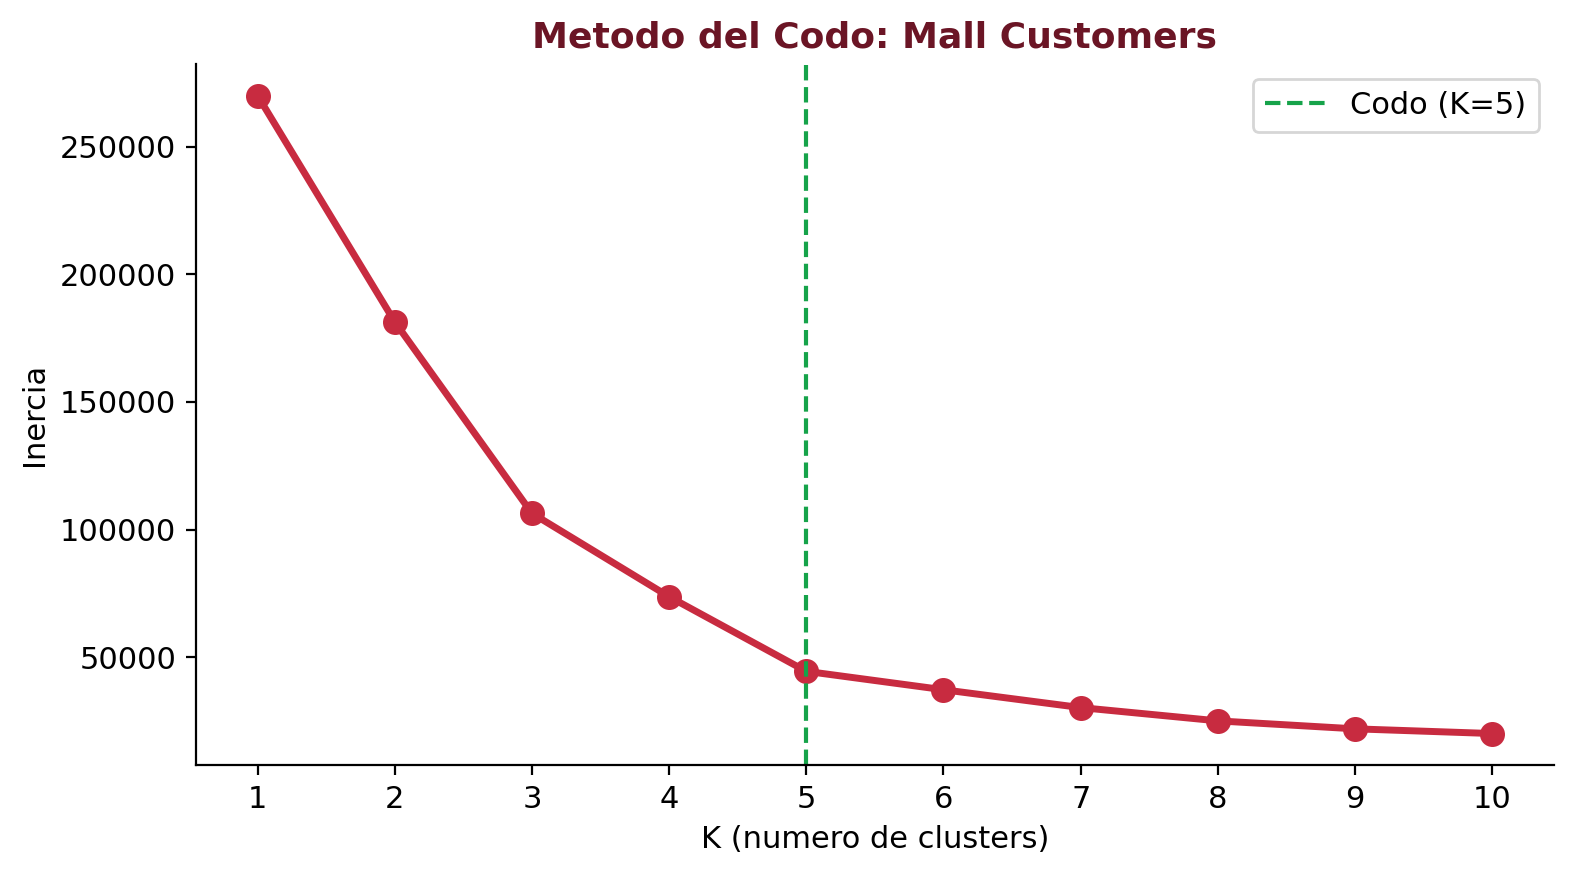
\includegraphics[width=0.78\textwidth]{fig_codo.png}
  \end{center}

  \vspace{-2pt}
  {\scriptsize\color{textMuted}
    \faLightbulb\hspace{4pt} La curva baja r\'apido de $K=1$ a $K=3$.
    Despu\'es de $K=3$, la mejora es marginal. El \textbf{codo}
    est\'a en $K=3$: es el n\'umero de clusters m\'as razonable.}
\end{frame}

\begin{frame}[fragile,shrink=18]{C\'odigo: El Codo}
  \vspace{-6pt}
  \begin{pyblock}
inertias = []
K_range = range(1, 11)
for k in K_range:
    km = KMeans(n_clusters=k, random_state=42, n_init=10)
    km.fit(X_scaled)
    inertias.append(km.inertia_)

fig = px.line(x=list(K_range), y=inertias,
    title="Metodo del Codo",
    labels={"x": "K (clusters)", "y": "Inercia"})
fig.update_layout(template="plotly_white")
fig.show()
  \end{pyblock}

  \vspace{4pt}
  {\scriptsize\color{arcaDark}
    \faKey\hspace{4pt} El codo no siempre es obvio. Es una gu\'ia, no una
    regla absoluta. Tambi\'en importa que los clusters tengan
    \textbf{sentido de negocio} (interpretables).}
\end{frame}

\begin{frame}[shrink=15]{Efecto de K: Pocos vs Muchos Clusters}
  \vspace{-4pt}
  \begin{center}
    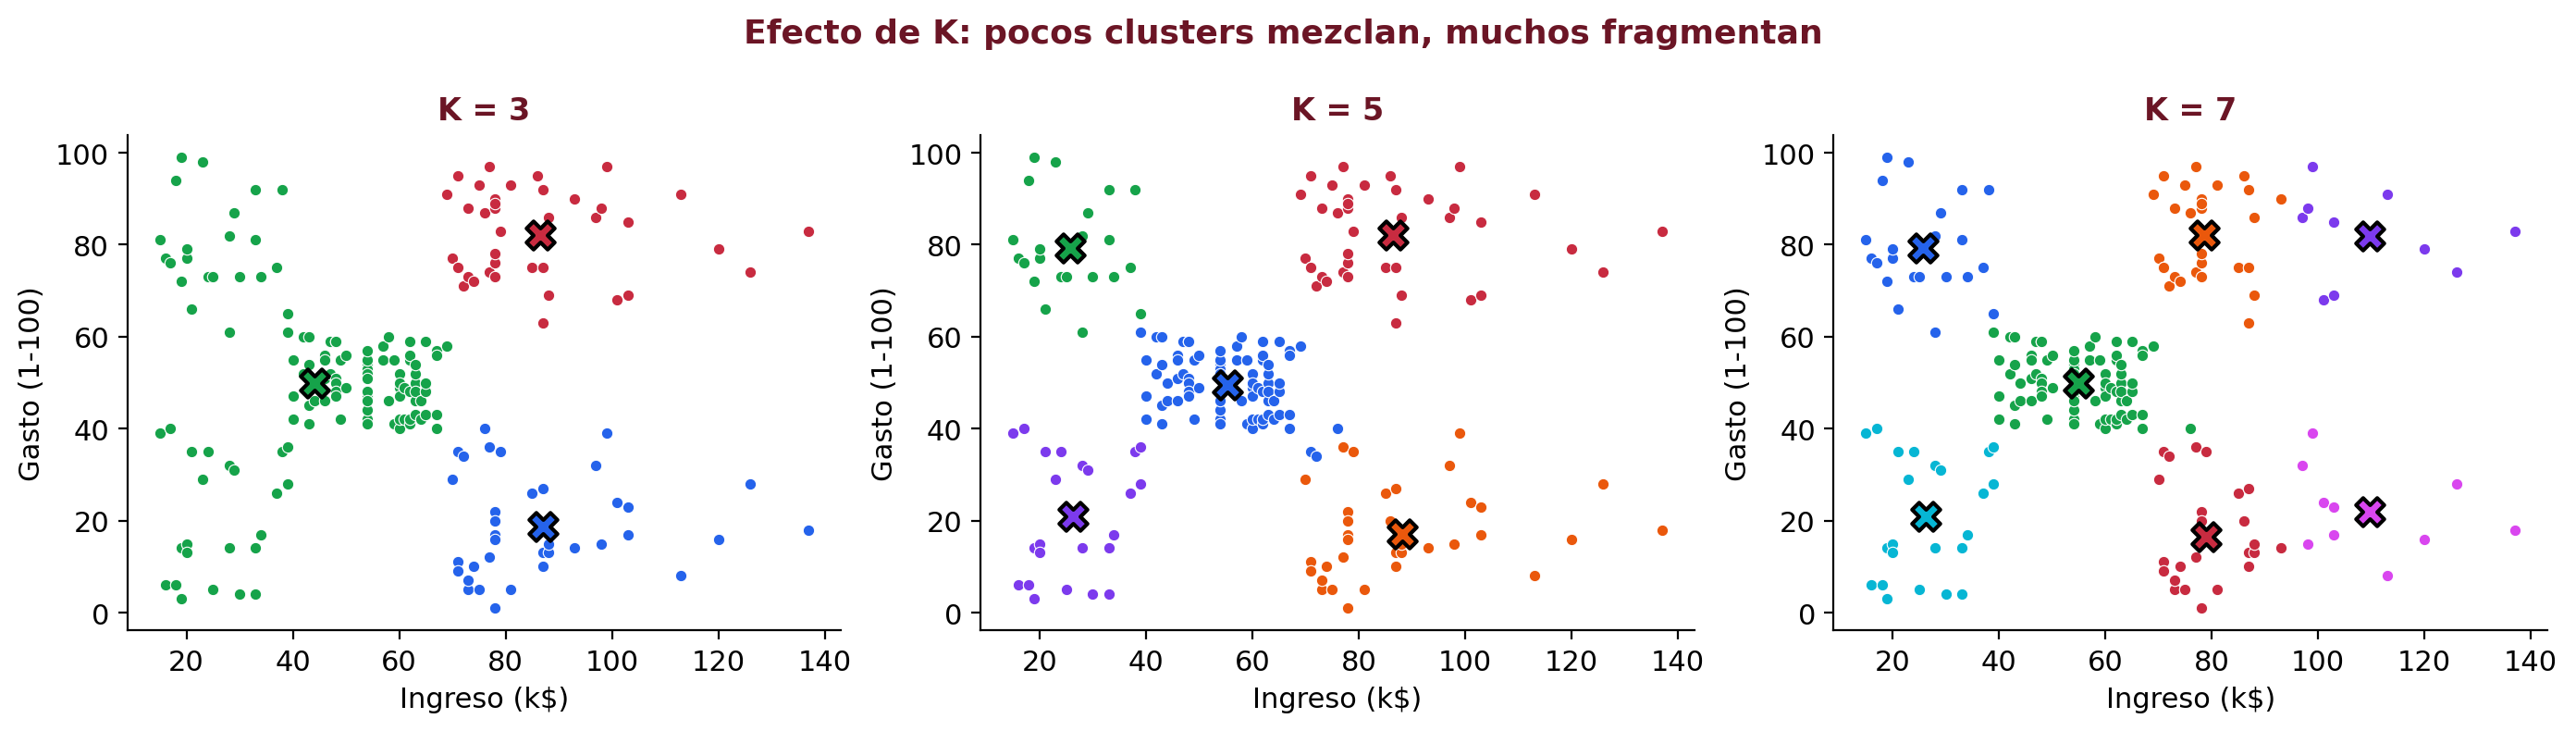
\includegraphics[width=0.88\textwidth]{fig_k_comparacion.png}
  \end{center}

  \vspace{-2pt}
  {\scriptsize\color{textMuted}
    \faLightbulb\hspace{4pt} $K=2$: mezcla grupos distintos.
    $K=3$: captura la estructura real.
    $K=5$: fragmenta grupos naturales en sub-grupos artificiales.
    M\'as clusters no siempre es mejor.}
\end{frame}

\begin{frame}{Silhouette Score --- ?`Qu\'e Tan Buenos Son los Clusters?}
  \vspace{-4pt}
  {\footnotesize\color{arcaDark}\bfseries
    El codo nos dice cu\'antos clusters usar, pero no nos dice
    \textbf{qu\'e tan bien separados} est\'an. Para eso existe
    el Silhouette Score.}

  \vspace{6pt}
  {\footnotesize
  \begin{itemize}\setlength{\itemsep}{5pt}
    \item[{\color{arcaRed}\scriptsize\faArrowRight}]
      Para cada punto, mide: ?`est\'a \textbf{m\'as cerca} de su propio
      cluster o del cluster vecino m\'as pr\'oximo?
    \item[{\color{arcaRed}\scriptsize\faArrowRight}]
      Rango: \textbf{$-1$} a \textbf{$+1$}.
      $+1$ = perfecto (muy dentro de su cluster).
      $0$ = en la frontera. $-1$ = probablemente en el cluster equivocado.
    \item[{\color{codeGreen}\scriptsize\faArrowRight}]
      El promedio de todos los puntos da un score global.
      Mayor de 0.5 se considera bueno. Mayor de 0.7, excelente.
  \end{itemize}
  }

  \vspace{4pt}
  {\scriptsize\color{textMuted}
    \faLightbulb\hspace{4pt} Podemos graficar Silhouette para cada $K$
    (igual que el codo) y elegir el $K$ con el score m\'as alto.}
\end{frame}

\begin{frame}[fragile,shrink=10]{C\'odigo: Silhouette Score}
  \vspace{-4pt}
  \begin{pyblock}
from sklearn.metrics import silhouette_score

for k in range(2, 8):
    km = KMeans(n_clusters=k, random_state=42, n_init=10)
    labels = km.fit_predict(X_scaled)
    sil = silhouette_score(X_scaled, labels)
    print(f"K={k}: Silhouette = {sil:.3f}")
  \end{pyblock}

  \vspace{4pt}
  {\scriptsize\color{arcaDark}
  \begin{itemize}\setlength{\itemsep}{3pt}
    \item[{\color{arcaRed}\scriptsize\faArrowRight}]
      \texttt{silhouette\_score} necesita m\'inimo $K=2$ (con 1 cluster
      no hay nada que comparar).
    \item[{\color{arcaRed}\scriptsize\faArrowRight}]
      Elegir el $K$ que tenga el \textbf{Silhouette m\'as alto}.
    \item[{\color{codeGreen}\scriptsize\faArrowRight}]
      Usar el codo \textbf{y} el Silhouette juntos: si ambos apuntan
      al mismo $K$, la elecci\'on es robusta.
  \end{itemize}
  }
\end{frame}

% =============================================================================
%  BLOQUE F: APLICACI\'ON MALL CUSTOMERS
% =============================================================================
\sectionframe{Aplicaci\'on}{Segmentar clientes de un centro comercial}

\begin{frame}{Mall Customers: El Dataset}
  \vspace{-4pt}
  {\footnotesize\color{arcaDark}\bfseries
    200 clientes de un centro comercial. Solo 3 variables:
    \textbf{ingreso anual}, \textbf{spending score} (qu\'e tanto gastan)
    y \textbf{edad}. No hay target --- no sabemos qu\'e ``tipo'' de
    cliente es cada uno.}

  \vspace{6pt}
  {\scriptsize
  \begin{tabular}{@{}llp{7cm}@{}}
    \toprule
    \textbf{Variable} & \textbf{Tipo} & \textbf{Descripci\'on} \\
    \midrule
    \texttt{income} & Continua & Ingreso anual (miles de d\'olares). \\
    \texttt{spending} & Continua & Spending Score (1--100): qu\'e tanto compra. \\
    \texttt{age} & Continua & Edad del cliente. \\
    \texttt{gender} & Categ\'orica & Male / Female. \\
    \bottomrule
  \end{tabular}
  }

  \vspace{6pt}
  \begin{tcolorbox}[colback=arcaGray, colframe=arcaRed, boxrule=0.5pt, arc=2pt,
    left=6pt, right=6pt, top=4pt, bottom=4pt]
    {\scriptsize\color{arcaDark}
    \faKey\hspace{4pt}\textbf{La pregunta de negocio:} ?`qu\'e tipos de clientes
    tenemos? ?`A qui\'en le hacemos campa\~nas de descuento y a qui\'en
    le ofrecemos productos premium? K-Means encuentra los segmentos.}
  \end{tcolorbox}
\end{frame}

\begin{frame}{?`Por Qu\'e Segmentar Clientes?}
  \vspace{-4pt}
  {\footnotesize\color{arcaDark}\bfseries
    Un gerente de marketing no hace la misma campa\~na para todos.
    Segmentar permite \textbf{personalizar} la estrategia:}

  \vspace{6pt}
  {\footnotesize
  \begin{itemize}\setlength{\itemsep}{5pt}
    \item[{\color{arcaRed}\scriptsize\faArrowRight}]
      Clientes con \textbf{alto ingreso y alto gasto}: ofrecerles
      productos premium, tarjeta VIP, experiencias exclusivas.
    \item[{\color{arcaRed}\scriptsize\faArrowRight}]
      Clientes con \textbf{alto ingreso pero bajo gasto}: oportunidad
      enorme --- tienen dinero pero no est\'an comprando. ?`Por qu\'e?
      Campa\~nas dirigidas.
    \item[{\color{arcaRed}\scriptsize\faArrowRight}]
      Clientes con \textbf{bajo ingreso y alto gasto}: cuidado ---
      pueden estar sobre-endeud\'andose. Programas de fidelizaci\'on.
    \item[{\color{codeGreen}\scriptsize\faArrowRight}]
      K-Means encuentra estos grupos \textbf{autom\'aticamente}
      a partir de los datos, sin que nosotros definamos las reglas.
  \end{itemize}
  }
\end{frame}

\begin{frame}[shrink=18]{Los 5 Segmentos que K-Means Encuentra}
  \vspace{-4pt}
  \begin{center}
    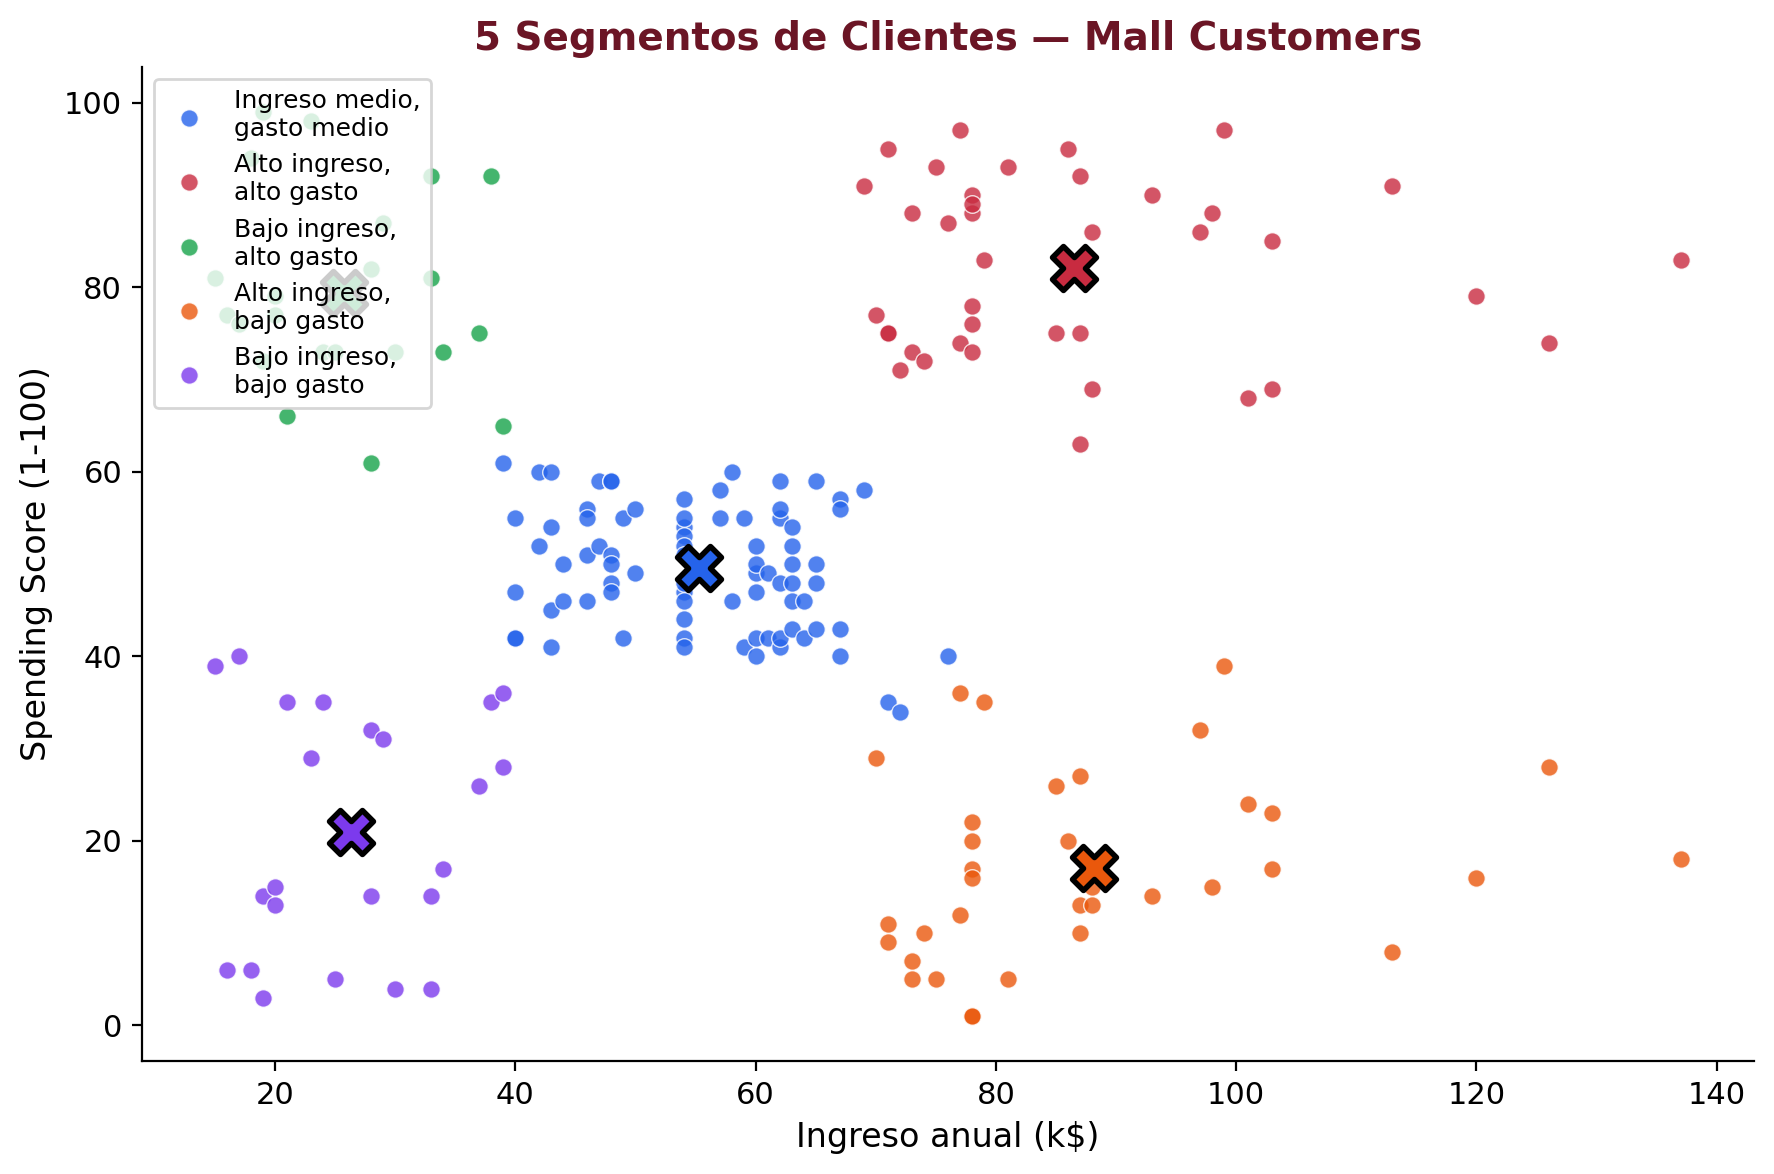
\includegraphics[width=0.78\textwidth]{fig_segmentos_mall.png}
  \end{center}

  \vspace{-2pt}
  {\scriptsize\color{textMuted}
    \faLightbulb\hspace{4pt} K-Means descubre 5 grupos claros en el espacio
    ingreso $\times$ gasto. Cada grupo es un \textbf{perfil de cliente}
    distinto. Los nombres los ponemos nosotros seg\'un el perfil.}
\end{frame}

\begin{frame}[fragile,shrink=22]{C\'odigo: Segmentar y Perfilar}
  \vspace{-6pt}
  \begin{pyblock}
import pandas as pd
from sklearn.cluster import KMeans

df = pd.read_csv("mall_customers.csv")
X = df[["Annual Income (k$)", "Spending Score (1-100)"]]

km = KMeans(n_clusters=5, random_state=42, n_init=10)
df["segmento"] = km.fit_predict(X)

# Perfilar: promedio de cada variable por segmento
perfil = df.groupby("segmento")[["Age", "Annual Income (k$)",
                    "Spending Score (1-100)"]].mean()
print(perfil.round(1))
  \end{pyblock}

  \vspace{4pt}
  {\scriptsize\color{arcaDark}
    \faKey\hspace{4pt} La tabla de perfiles convierte n\'umeros de cluster
    en \textbf{personas reales}: ``el segmento 2 tiene ingreso promedio
    de 86k y gasto de 82 --- son los clientes premium''.
    Eso es \'util para marketing.}
\end{frame}

% =============================================================================
%  BLOQUE G: INTERPRETAR CLUSTERS
% =============================================================================
\sectionframe{Interpretar los Clusters}{Darle sentido a los grupos}

\begin{frame}{El Paso M\'as Importante: Perfilar}
  \vspace{-4pt}
  {\footnotesize\color{arcaDark}\bfseries
    K-Means te dice \textbf{qu\'e} grupo, pero no \textbf{por qu\'e}.
    Perfilar = calcular el promedio de cada variable por cluster
    y darle un nombre interpretable.}

  \vspace{6pt}
  {\footnotesize
  \begin{itemize}\setlength{\itemsep}{5pt}
    \item[{\color{arcaRed}\scriptsize\faArrowRight}]
      \texttt{df.groupby("segmento").mean()} da los promedios.
    \item[{\color{arcaRed}\scriptsize\faArrowRight}]
      Comparar contra la media global: ?`este segmento tiene glucosa
      \textbf{por encima} o \textbf{por debajo} del promedio?
    \item[{\color{arcaRed}\scriptsize\faArrowRight}]
      Visualizar con \texttt{px.bar} agrupado o \texttt{px.scatter}
      coloreado por segmento.
    \item[{\color{codeGreen}\scriptsize\faArrowRight}]
      Darle un \textbf{nombre} a cada cluster:
      ``Bajo riesgo'', ``Riesgo metab\'olico'', ``Alto riesgo cl\'inico''.
  \end{itemize}
  }

  \vspace{4pt}
  {\scriptsize\color{textMuted}
    \faLightbulb\hspace{4pt} Un cluster sin interpretaci\'on es in\'util.
    El valor est\'a en la \textbf{acci\'on} que tomas con cada grupo,
    no en el n\'umero del cluster.}
\end{frame}

\begin{frame}[fragile,shrink=18]{Visualizar: Scatter Interactivo (Plotly)}
  \vspace{-6pt}
  \begin{pyblock}
fig = px.scatter(df, x="Annual Income (k$)",
    y="Spending Score (1-100)",
    color=df["segmento"].astype(str),
    size="Age", hover_data=["Gender"],
    title="Segmentos de clientes",
    color_discrete_sequence=["#2563EB","#C82B40","#16A34A",
                             "#EA580C","#7C3AED"])
fig.update_layout(template="plotly_white")
fig.show()
  \end{pyblock}

  \vspace{4pt}
  {\scriptsize\color{arcaDark}
    \faMousePointer\hspace{4pt} Pasen el mouse sobre cada punto:
    ven ingreso, gasto, edad y g\'enero. El tama\~no del punto
    representa la edad. Los colores son los segmentos.}
\end{frame}

\begin{frame}[shrink=5]{Ejercicio 2: Segmentar Iris \textbf{sin} Usar las Etiquetas}
  \vspace{-4pt}
  {\footnotesize\color{arcaDark}\bfseries
    \faClock\hspace{4pt} 15 minutos --- dataset Iris (\texttt{from sklearn.datasets import load\_iris}):}

  \vspace{6pt}
  {\footnotesize
  \begin{enumerate}\setlength{\itemsep}{4pt}
    \item Cargar Iris: \texttt{iris = load\_iris(as\_frame=True)}.
      Usar solo \texttt{iris.data} (las 4 medidas).
      \textbf{No miren} \texttt{iris.target} todav\'ia.
    \item Escalar con \texttt{StandardScaler} (4 variables en escalas distintas).
    \item M\'etodo del codo + Silhouette. ?`Cu\'antos clusters sugieren?
    \item Correr K-Means con ese $K$. Visualizar con \texttt{px.scatter}
      usando \texttt{petal length} vs \texttt{petal width} coloreado por cluster.
    \item \textbf{Ahora s\'i:} comparar sus clusters con las especies reales
      (\texttt{iris.target}). Hagan un \texttt{crosstab} entre cluster y especie.
    \item ?`K-Means recuper\'o las 3 especies sin saber que exist\'ian?
      ?`D\'onde se confunde?
  \end{enumerate}
  }
\end{frame}

\begin{frame}[shrink=5]{Ejercicio 3: Agregar Edad como Tercera Variable}
  \vspace{-4pt}
  {\footnotesize\color{arcaDark}\bfseries
    \faClock\hspace{4pt} 10 minutos:}

  \vspace{6pt}
  {\footnotesize
  \begin{enumerate}\setlength{\itemsep}{4pt}
    \item Repitan K-Means pero usando 3 variables: ingreso, gasto y edad.
    \item Recuerden escalar con \texttt{StandardScaler} (obligatorio).
    \item ?`Cambian los segmentos? ?`El codo sugiere un K distinto?
    \item Hagan un \texttt{px.scatter\_3d} con ingreso $\times$ gasto
      $\times$ edad coloreado por segmento.
    \item ?`La edad agrega informaci\'on \'util o solo agrega ruido?
  \end{enumerate}
  }

  \vspace{6pt}
  \begin{tcolorbox}[colback=arcaGray, colframe=arcaRed, boxrule=0.5pt, arc=2pt,
    left=6pt, right=6pt, top=4pt, bottom=4pt]
    {\scriptsize\color{arcaDark}
    \faKey\hspace{4pt} M\'as variables no siempre significa mejores clusters.
    A veces agregar variables ruidosas empeora la segmentaci\'on.
    Elegir las variables correctas es parte del trabajo del data scientist.}
  \end{tcolorbox}
\end{frame}

% =============================================================================
%  CIERRE
% =============================================================================
\sectionframe{Cierre}{Lo que aprendimos hoy}

\begin{frame}[shrink=10]{Resumen}
  \vspace{-4pt}
  \begin{columns}[T]
    \begin{column}{0.48\textwidth}
      {\footnotesize\bfseries\color{codePurple} Despliegue (Gradio):}
      \vspace{4pt}

      {\footnotesize
      \begin{itemize}\setlength{\itemsep}{3pt}
        \item[{\color{codeGreen}\faCheckCircle}]
          API = input $\to$ funci\'on $\to$ output.
        \item[{\color{codeGreen}\faCheckCircle}]
          Gradio: interfaz web en 5 l\'ineas.
        \item[{\color{codeGreen}\faCheckCircle}]
          Sliders, dropdowns, m\'ultiples outputs.
        \item[{\color{codeGreen}\faCheckCircle}]
          \texttt{share=True} para compartir.
      \end{itemize}
      }

      \vspace{4pt}
      {\footnotesize\bfseries\color{codeBlue} Todo el diplomado:}
      \vspace{4pt}

      {\footnotesize
      \begin{itemize}\setlength{\itemsep}{3pt}
        \item[{\color{codeBlue}\faCheckCircle}]
          Python, pandas, visualizaci\'on.
        \item[{\color{codeBlue}\faCheckCircle}]
          Regresi\'on, clasificaci\'on, evaluaci\'on.
        \item[{\color{codeBlue}\faCheckCircle}]
          \'Arboles, RF, tuning, CV.
        \item[{\color{codeGreen}\faCheckCircle}]
          \textbf{Clustering (hoy)}.
      \end{itemize}
      }
    \end{column}

    \begin{column}{0.48\textwidth}
      {\footnotesize\bfseries\color{arcaRed} Aprendizaje no supervisado:}
      \vspace{4pt}

      {\footnotesize
      \begin{itemize}\setlength{\itemsep}{3pt}
        \item[{\color{codeGreen}\faCheckCircle}]
          Sin target: descubrir estructura.
        \item[{\color{codeGreen}\faCheckCircle}]
          K-Means: asignar $\to$ recalcular $\to$ repetir.
        \item[{\color{codeGreen}\faCheckCircle}]
          Escalar es obligatorio.
        \item[{\color{codeGreen}\faCheckCircle}]
          Elegir K: m\'etodo del codo.
        \item[{\color{codeGreen}\faCheckCircle}]
          Interpretar: perfilar cada cluster.
        \item[{\color{codeGreen}\faCheckCircle}]
          Combinar con supervisado: clusters como features.
      \end{itemize}
      }
    \end{column}
  \end{columns}

  \vspace{6pt}
  \begin{tcolorbox}[colback=arcaRed!8, colframe=arcaRed, boxrule=0.5pt, arc=2pt,
    left=6pt, right=6pt, top=4pt, bottom=4pt]
    {\scriptsize\color{arcaDark}
    \faArrowRight\hspace{4pt}\textbf{Pr\'oxima clase:} Proyecto integrador
    --- aplicar todo lo aprendido a un problema real de principio a fin.}
  \end{tcolorbox}
\end{frame}

% ── QR ENCUESTA ──────────────────────────────────────────────────────────────
{
\setbeamertemplate{headline}{}
\setbeamertemplate{footline}{}
\begin{frame}[plain, noframenumbering]
  \begin{tikzpicture}[remember picture, overlay]
    \fill[arcaDark] (current page.south west) rectangle (current page.north east);
  \end{tikzpicture}
  \vspace{1cm}
  \begin{center}
    {\Huge\bfseries\color{white} ?`C\'omo estuvo la clase?\par}
    \vspace{0.6cm}
    
\includegraphics[width=4cm]{qr_encuesta.jpg}
    \vspace{0.4cm}

    {\large\color{white!80} Escanea el QR para dejarnos tu opini\'on.\par}
  \end{center}
\end{frame}
}

\end{document}
